\chapter{Introduction}
\section{Aims and objectives}
The aim of the project is to develop realistic spider animation that could be observed closely using the Oculus Rift. The result of the spider animation does not have to exactly follow the constraints of biology or physics, but should produce an animation which could deceive people to believe that it is real. 
The project will be divided into two main parts: animation and rendering. 
The most important part of the animation is the locomotion behavior which mainly handles the way in which the spider makes a step. 
There are three main general methods used to achieve this: keyframe animation, procedural animation and physical simulation. Usually, a keyframe method cannot tackle the task easily, since the keyframe animation mainly injects rules of attributes into a function of time. The physical animation is much more complex than procedural animation; as a result of this, the project will adopt a procedural method that mainly involves combining rules learned from biology or observation with kinematic animation.  
Since the project will adopt skeletal animation, it is required that a model of the spider is built before trying to animate it. Figure  \ref{fig:realSpider} is an image of a real wolf spider and Figure \ref{fig:spiderModel} is a similar model to the real wolf spider.
\begin{figure}[ht!]
\centering
\begin{minipage}[b]{0.45\linewidth}
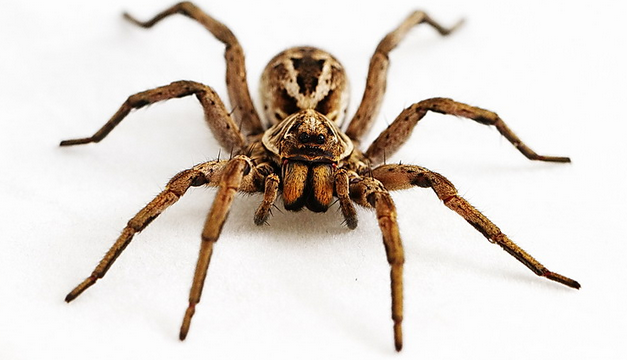
\includegraphics[width=7cm]{figures/realSpider.png}
\caption{A real wolf spider. \protect\cite{realSpider}}
\label{fig:realSpider}
\end{minipage}
\quad
\begin{minipage}[b]{0.45\linewidth}
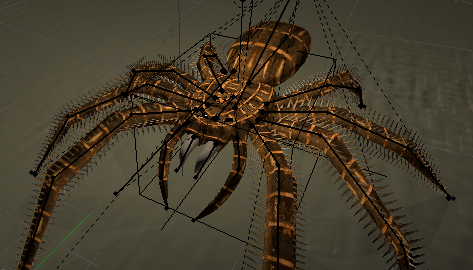
\includegraphics[width=7cm]{figures/spiderModel.png}
\caption{A wolf spider model \protect\cite{spiderModel}}
\label{fig:spiderModel}
\end{minipage}
\end{figure}
\cite{thesis} is a research about arthropod animation which implemented a hybrid approach. This includes procedural and physical approaches. The work of \cite{thesis} is based on the three locomotion layers proposed in \cite{steering}. \cite{steering} has divided the locomotion animation into three main parts: action selection, steering behavior and locomotion behavior. Thus the main objectives of the animation part is to implement the steering and locomotion behavior layers in \cite{steering}.
While the rendering part is also important due to the aim of observing the animation closely. A general texture mapping is not sufficient for the task as the close observation requires a considerable level of detail(e.g. fur of the spider). There are two methods specifically for rendering fur of an arthropod. These are side-view texture mapping and fins and shells techniques\cite{fur}. However, due to the limited time of the project, initially only polygon meshes or simple texture mapping will be considered.
The Oculus Rift is a virtual reality headset developed by Oculus VR. It enables users to seamlessly look around the virtual world. It tracks every little movement of users' head to create a natural experience \cite{rift1}. Figure \ref{fig:rift} is an image of device Oculus Rift 2.
\begin{figure}[ht!]
\centering
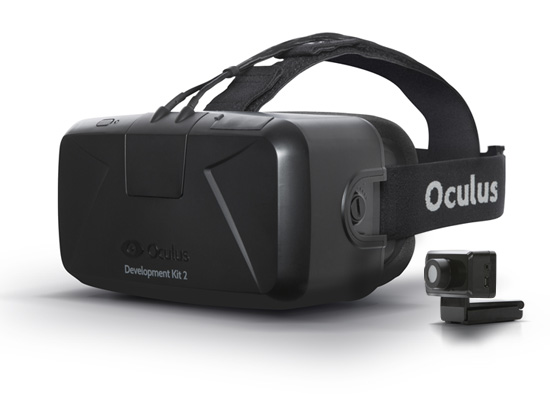
\includegraphics[height=8cm]{figures/rift.jpg}
\caption{Oculus Rift 2. \protect\cite{rift1}}
\label{fig:rift}
\end{figure}
\section{Overview of the report}
The remaining report is structured as follows: 
\begin{itemize}
  \item \textbf{Chapter 2} will review previous research and techniques relevant to this project. This chapter will also discuss general animation techniques. Then animation and rendering techniques specifically for arthropods will be covered.
  \item \textbf{Chapter 3} will analyze the aims of the project and divide the project into manageable subtasks. Evaluation criteria is also included in this chapter. 
  \item \textbf{Chapter 4} will give a plan about how the project will be done based on possible solutions proposed in Chapter 3. Risk analysis and possible countermeasures will also be included in this chapter.
  \item \textbf{Chapter 5} will draw a conclusion that briefly summarizes work done for the background report and the future work according to the plan proposed in Chapter 4.
\end{itemize}
